\section{Episodic Logic (EL)}
\label{sec:el}

EL is a predicate logic whose semantics are intended to model some important aspects of natural language, and of the human thought patterns that give rise to natural language.  As its name implies, one of EL's most distinctive features is its \textit{characterization} operator, \texttt{**}, which relates possible situations (a.k.a. \textit{episodes}, which include what we would informally call events) to the logical propositions that characterize them. EL also maps predicate and propositional intensions to \textit{individuals} within its logical domain; these intensional individuals are formed from EL's predicates and propositions using reification operators. Proposition intensions, when reified to individuals, can act as arguments to intensional verb predicates, e.g. \textit{believe} and \textit{refer (to)}. Predicate intensions can also be type-shifted into complex predicate \textit{modifiers}, e.g. \textit{hopefully believable}. EL also avoids a Montague-style treatment of determiners as second-order predicates, instead providing generalized, restricted quantifiers, including nonstandard quantifiers, e.g. \textit{most of the older boys}.

\begin{figure}
    \centering
    \scalebox{0.9}{
    \vbox{
    % Made with matchcha.io---strong recommendation from me! :)

%\epigraph{\textit{There are more things in heaven and earth, Horatio, Than are dreamt of in your philosophy.}}{---William Shakespeare, \textit{Hamlet}}

\tikzset{every picture/.style={line width=0.75pt}} %set default line width to 0.75pt        

\begin{center}
\scalebox{1.0}{
\makebox[\textwidth][c]{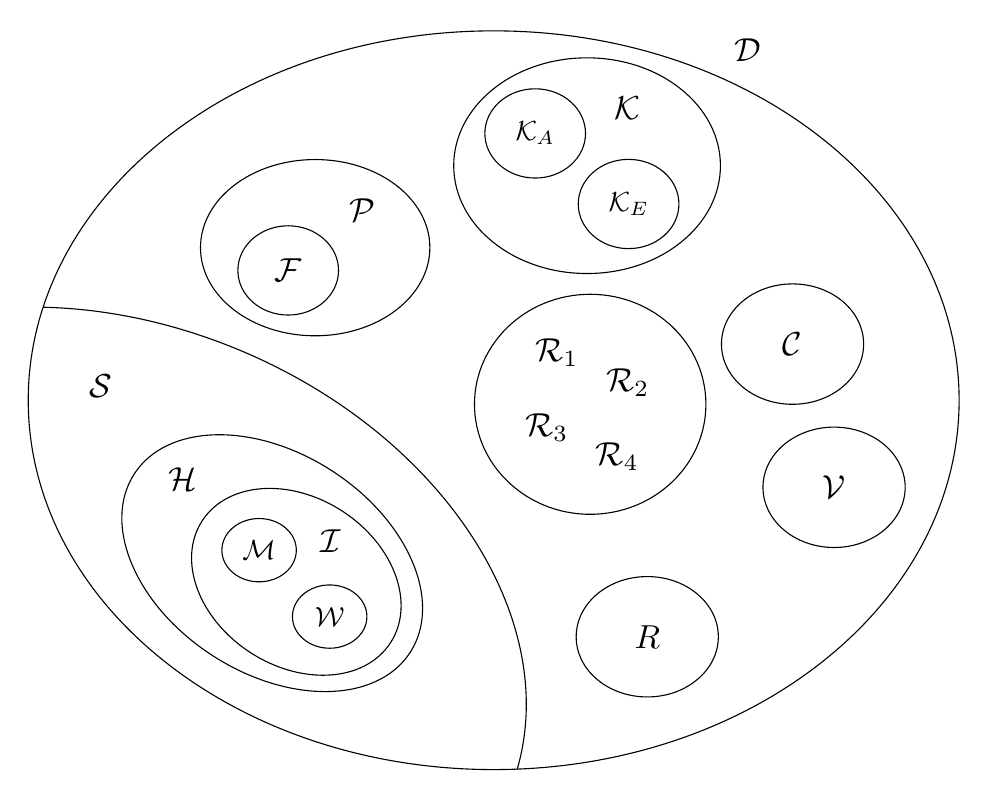
\begin{tikzpicture}[x=0.75pt,y=0.75pt,yscale=-1,xscale=1,scale=1,every node/.style={scale=1}]
%uncomment if require: \path (0,721.921875); %set diagram left start at 0, and has height of 721.921875

%Shape: Ellipse [id:dp9100065238827619] 
\draw   (98,300.96) .. controls (98,202.68) and (198.4,123) .. (322.25,123) .. controls (446.1,123) and (546.5,202.68) .. (546.5,300.96) .. controls (546.5,399.25) and (446.1,478.92) .. (322.25,478.92) .. controls (198.4,478.92) and (98,399.25) .. (98,300.96) -- cycle ;
%Shape: Ellipse [id:dp10388374342633644] 
\draw   (181,227.46) .. controls (181,204.01) and (205.74,185) .. (236.25,185) .. controls (266.76,185) and (291.5,204.01) .. (291.5,227.46) .. controls (291.5,250.91) and (266.76,269.92) .. (236.25,269.92) .. controls (205.74,269.92) and (181,250.91) .. (181,227.46) -- cycle ;
%Shape: Ellipse [id:dp27736097111625835] 
\draw   (199,238.42) .. controls (199,226.55) and (209.86,216.92) .. (223.25,216.92) .. controls (236.64,216.92) and (247.5,226.55) .. (247.5,238.42) .. controls (247.5,250.3) and (236.64,259.92) .. (223.25,259.92) .. controls (209.86,259.92) and (199,250.3) .. (199,238.42) -- cycle ;
%Shape: Ellipse [id:dp7888799168086817] 
\draw   (303,187.96) .. controls (303,159.26) and (331.77,136) .. (367.25,136) .. controls (402.73,136) and (431.5,159.26) .. (431.5,187.96) .. controls (431.5,216.66) and (402.73,239.92) .. (367.25,239.92) .. controls (331.77,239.92) and (303,216.66) .. (303,187.96) -- cycle ;
%Shape: Ellipse [id:dp4804121479534271] 
\draw   (363,206.42) .. controls (363,194.55) and (373.86,184.92) .. (387.25,184.92) .. controls (400.64,184.92) and (411.5,194.55) .. (411.5,206.42) .. controls (411.5,218.3) and (400.64,227.92) .. (387.25,227.92) .. controls (373.86,227.92) and (363,218.3) .. (363,206.42) -- cycle ;
%Shape: Ellipse [id:dp0795716353230258] 
\draw   (318,172.42) .. controls (318,160.55) and (328.86,150.92) .. (342.25,150.92) .. controls (355.64,150.92) and (366.5,160.55) .. (366.5,172.42) .. controls (366.5,184.3) and (355.64,193.92) .. (342.25,193.92) .. controls (328.86,193.92) and (318,184.3) .. (318,172.42) -- cycle ;
%Shape: Ellipse [id:dp12618348576003102] 
\draw   (432,273.92) .. controls (432,257.91) and (447.33,244.92) .. (466.25,244.92) .. controls (485.17,244.92) and (500.5,257.91) .. (500.5,273.92) .. controls (500.5,289.94) and (485.17,302.92) .. (466.25,302.92) .. controls (447.33,302.92) and (432,289.94) .. (432,273.92) -- cycle ;
%Shape: Ellipse [id:dp8799691211755756] 
\draw   (452,342.92) .. controls (452,326.91) and (467.33,313.92) .. (486.25,313.92) .. controls (505.17,313.92) and (520.5,326.91) .. (520.5,342.92) .. controls (520.5,358.94) and (505.17,371.92) .. (486.25,371.92) .. controls (467.33,371.92) and (452,358.94) .. (452,342.92) -- cycle ;
%Shape: Ellipse [id:dp824996442524188] 
\draw   (362,414.92) .. controls (362,398.91) and (377.33,385.92) .. (396.25,385.92) .. controls (415.17,385.92) and (430.5,398.91) .. (430.5,414.92) .. controls (430.5,430.94) and (415.17,443.92) .. (396.25,443.92) .. controls (377.33,443.92) and (362,430.94) .. (362,414.92) -- cycle ;
%Shape: Ellipse [id:dp8272383634329143] 
\draw   (313,302.92) .. controls (313,273.65) and (337.96,249.92) .. (368.75,249.92) .. controls (399.54,249.92) and (424.5,273.65) .. (424.5,302.92) .. controls (424.5,332.19) and (399.54,355.92) .. (368.75,355.92) .. controls (337.96,355.92) and (313,332.19) .. (313,302.92) -- cycle ;
%Shape: Arc [id:dp39537977602891705] 
\draw  [draw opacity=0] (105.32,256.16) .. controls (135.93,256.87) and (168.45,263.64) .. (200.4,277.07) .. controls (297.72,317.98) and (354.69,406) .. (333.59,478.73) -- (143.5,412.42) -- cycle ; \draw   (105.32,256.16) .. controls (135.93,256.87) and (168.45,263.64) .. (200.4,277.07) .. controls (297.72,317.98) and (354.69,406) .. (333.59,478.73) ;
%Shape: Ellipse [id:dp5287011551360823] 
\draw   (149.07,336.49) .. controls (164.96,311.91) and (207.6,311.22) .. (244.32,334.95) .. controls (281.04,358.69) and (297.92,397.86) .. (282.03,422.44) .. controls (266.14,447.02) and (223.49,447.71) .. (186.77,423.97) .. controls (150.06,400.24) and (133.18,361.07) .. (149.07,336.49) -- cycle ;
%Shape: Ellipse [id:dp015166695228427951] 
\draw   (181.78,359.11) .. controls (193.96,340.26) and (224.16,338.12) .. (249.23,354.32) .. controls (274.3,370.53) and (284.75,398.94) .. (272.56,417.79) .. controls (260.38,436.64) and (230.18,438.78) .. (205.11,422.58) .. controls (180.04,406.37) and (169.59,377.96) .. (181.78,359.11) -- cycle ;
%Shape: Ellipse [id:dp4822793325306267] 
\draw   (191.3,373.21) .. controls (191.3,364.79) and (199.33,357.96) .. (209.23,357.96) .. controls (219.14,357.96) and (227.17,364.79) .. (227.17,373.21) .. controls (227.17,381.63) and (219.14,388.45) .. (209.23,388.45) .. controls (199.33,388.45) and (191.3,381.63) .. (191.3,373.21) -- cycle ;
%Shape: Ellipse [id:dp37988107849014874] 
\draw   (225.3,405.21) .. controls (225.3,396.79) and (233.33,389.96) .. (243.23,389.96) .. controls (253.14,389.96) and (261.17,396.79) .. (261.17,405.21) .. controls (261.17,413.63) and (253.14,420.45) .. (243.23,420.45) .. controls (233.33,420.45) and (225.3,413.63) .. (225.3,405.21) -- cycle ;

% Text Node
\draw (133,294) node [scale=1.2]  {$\mathcal{S}$};
% Text Node
\draw (244,369) node [scale=1.2]  {$\mathcal{I}$};
% Text Node
\draw (209.23,373.21) node [scale=1]  {$\mathcal{M}$};
% Text Node
\draw (243.23,405.21) node [scale=1]  {$\mathcal{W}$};
% Text Node
\draw (172.23,339.21) node [scale=1.2]  {$\mathcal{H}$};
% Text Node
\draw (396.25,414.92) node [scale=1.2]  {$\mathbb{R}$};
% Text Node
\draw (352.8,278.27) node [scale=1.2]  {$\mathcal{R}_{1}$};
% Text Node
\draw (386.8,292.27) node [scale=1.2]  {$\mathcal{R}_{2}$};
% Text Node
\draw (347.8,314.27) node [scale=1.2]  {$\mathcal{R}_{3}$};
% Text Node
\draw (381.8,328.27) node [scale=1.2]  {$\mathcal{R}_{4}$};
% Text Node
\draw (386.8,160.27) node [scale=1.2]  {$\mathcal{K}$};
% Text Node
\draw (342.25,172.42) node [scale=1]  {$\mathcal{K}_{A}$};
% Text Node
\draw (387.25,206.42) node [scale=1]  {$\mathcal{K}_{E}$};
% Text Node
\draw (466.25,273.92) node [scale=1.2]  {$\mathcal{C}$};
% Text Node
\draw (486.25,342.92) node [scale=1.2]  {$\mathcal{V}$};
% Text Node
\draw (258.8,209.27) node [scale=1.2]  {$\mathcal{P}$};
% Text Node
\draw (223.25,238.42) node [scale=1.2]  {$\mathcal{F}$};
% Text Node
\draw (444.8,132.27) node [scale=1.2]  {$\mathcal{D}$};


\end{tikzpicture}}}
\end{center}

\small
\makebox[\textwidth][c]{\begin{tabular}{c c l}
   & & \\
   $\mathcal{D}$  & & The full \textit{domain} of EL individuals; the union of all following sets \\
   $\mathcal{S}$  & & Possible situations, a.k.a. \textit{episodes}, forming a join semilattice in any given possible world \\
   $\mathcal{H}$  & & Informationally-maximal episodes, a.k.a. \textit{exhaustive situations} \\
   $\mathcal{I}$  & & Spatially-maximal exhaustive situations, a.k.a. \textit{possible times}, a.k.a intervals \\
   $\mathcal{W}$  & & Spatiotemporally-maximal intervals, a.k.a. \textit{possible worlds} \\
   $\mathcal{M}$  & & Spatially-maximal, temporally-minimal intervals, a.k.a. \textit{moments of time} \\
   $\mathcal{P}$  & & \textit{Propositions} \\
   $\mathcal{F}$  & & Consistent propositions, a.k.a. \textit{possible facts} \\
   $\mathcal{K}$  & & \textit{Kinds of individuals}, whose realizations are ordinary individuals \\
   $\mathcal{K}_{A}$  & & \textit{Kinds of actions}, whose realizations are pairs of ordinary individuals and situations \\
   $\mathcal{K}_{E}$  & & \textit{Kinds of episodes}, whose realizations are situations for which a particular characterization holds \\
   $\mathcal{C}$  & & \textit{Collections} of individuals \\
   $\mathcal{V}$  & & \textit{$n$-tuples} of individuals, $n \geq 2$ \\
   $\mathbb{R}$  & & \textit{The real numbers} \\
   $\mathcal{R}_{1}$  & & \textit{Clock times, a uniformly discretized subset of $\mathbb{R}$}, containing subsets of $\mathbb{R}_{n}$
   %& & Note that $\mathcal{R}_{4}$, which represents space-time regions, contains some unconnected \\
   %& & space-time trajectories; these trajectories describe the time and place of episodes.
\end{tabular}}
    }
    }

    \caption{A representation of the EL ontology. I include only some brief definitions of its notable subsets; for more formal detail, please refer to \citep{schubert2000episodic}.}% \tiny{(I'd like to thank \href{https://www.mathcha.io}{mathcha.io} for making the construction of this TikZ figure so painless with their graphical editor.)}}
    \label{fig:el_ontology}
\end{figure}

The EL ontology of individuals, represented by Figure~\ref{fig:el_ontology}, gives a hierarchical organization of the basic semantic types of EL. The \textit{kind-forming} operators---$\texttt{K}$ (kind), $\texttt{KA}$ (kind of action), and $\texttt{KE}$ (kind of event)---reify predicates and propositions into the respectively named types in the ontology. EL defines a variety of semantic types, such as those for predicates and modifiers, on the basis the domain of individuals $\mathcal{D}$, and the set of truth values, $\{0,1\}$, also written as \textbf{2}. These semantic types are compositions of mapping functions, each of which is notated $(X \rightarrow Y)$ to mean a function mapping set $X$ to set $Y$. For example, the monadic noun predicate \texttt{STEAK.N}, denoting the set of individuals that are steak, has semantic type $(\mathcal{D} \rightarrow (\mathcal{S} \rightarrow \textbf{2}))$: it is a mapping of individuals to mappings of \textit{situations} to truth values, thereby affording intensionality. $n$-adic predicates generally have the type $(\mathcal{D}^{n} \rightarrow (\mathcal{S} \rightarrow \textbf{2}))$. Semantic types in EL may be re-cast using \textit{type-shifting} operators, e.g. the reifying operator \texttt{K}, a.k.a. the \textit{kind} operator, which maps a monadic predicate into a ``kind of'' individual and has semantic type $((\mathcal{D} \rightarrow (\mathcal{S} \rightarrow \textbf{2})) \rightarrow \mathcal{K})$.

\subsection{Examination of an Example}
In lieu of formal, detailed definitions of all of EL's features, which can be found in \citep{schubert2000episodic} \footnote{modulo a redefinition of the semantics of the characterizing operator, \el{**}, in terms of the underlying predicate semantics \citep{len-situations-2000} instead of the semantics of the truth-in operator, \el{*}}, the remainder of this section is dedicated to the examination of an example of an English/EL pair that illustrates some of those most notable features. Everything heretofore written in this section will refer to the formula in Figure~\ref{fig:eng_el_pair}.

\subsubsection{The \el{**} operator}
Two propositions \textit{characterize} event individuals in the example formula: the \el{insist.v} proposition, which characterizes \el{e1.sk}, and the \el{like.v} proposition, which characterizes \el{e2}. When a formula $\phi$ characterizes an episode \el{e}, it means that \el{e} is \textit{an episode of} $\phi$; we write this relationship as \el{($\phi$ ** e)}. The characterization of episode individuals by formulas is similar to the Davidsonian notion of events \citep{Davidson1967}, where an event is a first-class domain entity passed as an extra argument to situational predicates. Davidsonian event variables, however, may only passed to positive, atomic predications; Episodic Logic's semantics allow arbitrarily complex formulas to characterize, and thus to hold in certain events.

\el{**} is a \textit{modal} operator: statements like \el{[$\phi$ ** e]} may not, in general, have their formula argument, $\phi$, replaced with other formulas that seem to have the same truth value. So, the EL formula \el{((|Andre| sleep.v) ** e)} does \textit{not} entail \el{(((|Andre| sleep.v) $\land$ ( (|Fido| bark.v) $\lor$ $\neg$ (|Fido| bark.v) )) ** e)}, even though it has the same truth value; in fact, the entity \el{|Fido|} might not have any role in the episode, and so even tautological statements involving it may have no truth value in \el{e}.

\begin{figure}

\textbf{English}: \textit{Most of the senior students will insist that they liked art.}

\textbf{EL}: \begin{lstlisting}[xleftmargin=4.5em,style=EL,mathescape=true]
(e1.sk after Now) $\land$
(most.det x [(x student.n) $\land$ (x senior.a)]
    ((x insist.v (that 
        ($\exists$ e2 [e2 before e1.sk]
            ( (x like.v (k art.n)) ** e2 )
                ))) ** e1.sk))
\end{lstlisting}
    \caption{An example of an English sentence and its EL interpretation. There is no difference, here, between square brackets and parentheses; they alternate only to make distinguishing certain clauses easier. Note that, in this notation, each subject argument \textit{precedes} its predicates, while all other arguments follow the predicate. In the ``curried'' semantics, subject arguments come last.}
    \label{fig:eng_el_pair}
\end{figure}

\subsubsection{Restricted quantification}
The existential quantification of \el{e2}\footnote{e1.sk, on the other hand, is a Skolem constant---it has been assigned a name to remove the top-level existential quantification of \el{e1}.\el{e2} could not be similarly Skolemized, as it is within the scope of the intensional predicate \texttt{insist.v}. Even without this intensional scope, though, \el{e2} would still have a subscope dependency on the quantified value of \el{x}, i.e., \el{e2} would be a Skolem function of \el{x}.} illustrates the ``restrictor-matrix'' structure of EL quantification: if \el{x} is a variable, \el{Q} is a quantifier, and $\phi$ and $\psi$ are arbitrary EL formulas, the quantification formula \el{[Q x : $\phi$ $\psi$]} predicates the truth of the ``matrix'' formula $\psi$ in quantification cases where the ``restrictor'' formula $\phi$ holds true. When \el{Q} is $\exists$, this is equivalent to the unrestricted quantification \el{[$\exists$ x ($\phi \land \psi$)]}; similarly, when \el{Q} is $\forall$, it is equivalent to \el{[$\forall$ x ($\phi \rightarrow \psi$)]}. However, as can be seen in the quantification of \el{x} by the quantifier \el{most.det}, not all quantifiers can be simplified in this way: nonstandard quantifiers like \textit{most}, \textit{many}, and \textit{few} do not permit conjunctive or implicative re-writing of the restrictor formula.

\subsubsection{Temporal relations}
The temporal relation \el{before} is used to relate the time of \el{e1.sk} to the special time constant \el{now}---which represents the time that the speaker is uttering the sentence---and the time of \el{e2} to \el{e1.sk}, and thus also \el{e2} to \el{now}.
As \el{now} is indexical by default, if more than one utterance exists, we ``timestamp'' each utterance's \el{now}, e.g. \el{Now1}.
Such temporal relations---as well as the tacit temporal relations in their transitive closures---allow projection of the episodes onto temporal intervals within the ontological domain $\mathcal{R}_{1}$, representing discretized times (see Figure~\ref{fig:el_ontology}).
%Not all spacetime trajectories are transitively connected, however; the intensional environment of the verb predicate \el{insist.v} implies a new set of possible situations for the truth of the \el{like.v} proposition characterizing \el{e2}.

More temporal relations exist, special functions \el{start-of(e)} and \el{end-of(e)} allow temporal predications about the instantaneous endpoints of episodes, and disjoint intervals may even form an episode (e.g. \textit{Andre sneezed repeatedly}); for more information on the temporal semantics of EL, please refer to the original semantics due to \citet{hwang1993episodic} and their revisions by \citet{len-situations-2000}.

\subsubsection{Reification and \textit{kind}-forming}
The kind-forming operator \el{K} is used here because \el{art.n} is a one-place predicate that determines whether its argument is ``art''. Because the speaker does not have any specific art in mind, we choose to make a statement about the students liking the \textit{kind of thing} ``art'', which we accomplish by \textit{reifying} the \el{art.n} predicate, rather than \textit{Skolemizing} a variable (i.e. assigning it a concrete name, to bypass existential quantification) and attaching the predicate to it (i.e. assigning it a name). In order to use a predicate as an argument to another predicate, we must first reify it as an individual.

Reification can also be performed on other types of predicates. The reified verb phrase \el{(Ka (drink.v (K water.n)))}
%\footnote{What's being reified is actually not a well-formed EL predication, assuming \el{drink.v} is a 2-place predicate; the actor argument is missing! What's \textit{actually} being reified here, implicitly using the \el{K} operator, is something like the \textit{lambda abstraction} \el{($\lambda$a (a drink.v (K water.n)))}; however, even that's not quite right, as there are additional complications related to event characterization. For a full discussion of this, see page 7 of \citep{schubert2000episodic}.}
is the \textit{kind of action} of drinking water, and belongs to the class $\mathcal{K}_{A}$ in the EL ontology (see Figure~\ref{fig:el_ontology}), whose realizations are (individual, episode) pairs.
What's being reified by the \el{Ka} operator is a well-formed monadic EL predication, assuming \el{drink.v} is a 2-place ``curried'' predicate; \el{Ka} can be defined in terms of the \el{K} operator as \el{(K ($\lambda$a (((1st a) drink.v (K water.n)) ** (2nd a))))}, which is a kind whose realizations \el{a} have an agent as the first element and an episode as the second element. \footnote{see page 7 of \citep{schubert2000episodic}}
The reified sentence \el{(Ke (|Mary| drink.v (K water.n)))} is the \textit{kind of event} where Mary drinks water, and belongs to the ontological class $\mathcal{K}_{E}$. The \el{Ke} operator can also be defined in terms of the \el{K} operator: \el{(Ke $\phi$)} = \el{(K $\lambda$e ($\phi$ ** e))}. \el{Ke}-reification is semantically distinct from the other reification of this sentence, which uses the \el{That} operator, \el{(That (|Mary| drink.v (K water.n)))}, which is a \textit{proposition}, and thus belongs to the ontological class $\mathcal{P}$. An intuition for their semantic distinction is quite easy to obtain from the names of their operators: ``the kind of event of Mary drinking water'' is obviously different from the proposition ``that Mary is drinking water''.
%However, the restrictor-matrix form cannot be simplified in this manner for some of EL's nonstandard quantifiers, e.g. \el{Most}.
%As its name implies, one of EL's most distinctive features is its use of \textit{episode} variables to denote time-bounded ``temporal'' propositions, such as ``Palutena is sleepy'' or ``I'll go running for an hour''---as well as ``atemporal'' propositions, which necessarily hold true eternally, like ``hydrogen is an element'' or $2+3=5$.

%EL naturally supports other aspects of natural language as well. It is an \textit{intensional} logic: a sentence like ``Gaurav loves Mariel'' can represented as not just a truth value, but as a function from possible situations to truth values called a \textit{sentence intension}. Sentence intensions may be transmuted into individuals using \textit{reification} operator \texttt{That}, and predicates may be similarly reified into individuals with the kind-forming operator \texttt{K}\footnote{Or \texttt{Ke} for forming kinds of events, or \texttt{Ka} for forming kinds of actions.}; this allows abstract entities, such as \textit{``the process of writing a dissertation''}, as well as concrete entities, such as \textit{``Lane's dissertation''}, to act as predicate arguments without defining special semantics for higher-order predicates (that is, predicates with predicate arguments).